\documentclass[11pt]{utalcaDoc}
\usepackage{alltt}
\usepackage{underscore}
\usepackage[utf8]{inputenc}
\usepackage[activeacute,spanish]{babel}
\usepackage{verbatim}
\usepackage[pdftex]{graphicx}
\usepackage{ae}
\usepackage{amsmath}
\usepackage{amsfonts}
\usepackage{pdflscape}
\usepackage{inconsolata}
\usepackage{url}
\usepackage{hyperref}
\usepackage{listings}
% \usepackage{placeins}
\usepackage[section]{placeins}
\usepackage[stable]{footmisc}
\usepackage{minted}

\title{{\bf Seguridad Informática}\\ Laboratorio 1}
\author{Erik Regla\\ eregla09@alumnos.utalca.cl}
\date{\today}

\begin{document}
\maketitle
\newpage
\section{Introducción}
\section{Actividades}
\subsection{Cree un volumen encriptado, en un archivo, mediante la herramienta Veracrypt, utilizando una contraseña compleja y un archivo tipo keyfile. ¿Qué sucede cuando intenta ver el contenido del archivo generado desde una aplicación para visualizar archivos de texto?}

\begin{minted}{bash}
	#/bin/bash

	## installation of veracrypt
	sudo add-apt-repository ppa:unit193/encryption
	sudo apt update
	sudo apt install -y veracrypt
	
	## Generate keyfile
	veracrypt --create-keyfile #interactive
	
	## Volume creation
	## Use 10M as size
	PASSWORD="eKPClTK+IfHEBAASaUfCBWis0Y143h2i7uLM3ly+7PM="
	veracrypt -t -c --volume-type=normal ./enc_volume --encryption=aes \
	--hash=sha-512 --filesystem=ext4 -p $PASSWORD --pim=0 -k ./keyfile \
	--random-source=/dev/urandom  --size=10M
\end{minted}

Solo se ve basura. Ahora esa basura que hay es un archivo generado de manera aleatoria el cual es utilzado para poder decriptar el volumen.

\subsection{Genere un volumen encriptado utilizando una contraseña compleja y un archivo keyfile. Realice un respaldo de cabecera de dicho volumen. Posterior a esto, agregue un archivo al volumen creado y cambie la contraseña. Luego restaure el volumen utilizando el respaldo creado. ¿Los datos almacenados sufrieron algún cambio?}
Ninguno.


\begin{minted}{bash}
	## mount encrypted
	mkdir -p mnt
	veracrypt -t -k ./keyfile -p $PASSWORD --pim=0 --protect-hidden=no \ 
	./enc_volume ./mnt/
	
	## read keyfile
	cat ./keyfile
	
	## backup and see if it works
	cp enc_volume enc_volume.bkp
	sudo bash -c ' echo "basurita" > mnt/basura'
	sudo bash -c ' ls -alh mnt'
	veracrypt -d ./mnt
	rm -rfv enc_volume
	mv enc_volume.bkp enc_volume
	veracrypt -t -k ./keyfile -p $PASSWORD --pim=0 --protect-hidden=no\ 
	./enc_volume ./mnt/
	sudo bash -c ' ls -alh mnt'
	veracrypt -d ./mnt
\end{minted}

\subsection{Cree un volumen encriptado oculto. Utilice para volumen externo solo una contraseña y algoritmo de cifrado AES. Agregue durante la creación un archivo cualquiera para este volumen. Para el volumen oculto utilice un algoritmo de cifrado y hash diferente al anterior, utilice una contraseña compleja y un archivo de texto con la frase “Seguridad Informática 2020” como keyfile. Monte el volumen y observe que sucede.}


\begin{minted}{bash}
	## Create hidden volume
	PASSWORD_HIDDEN="q7AakbEP/kjSGcnpy6JbaNbXFtFD5wII+lrnJAHfnfo="
	echo "Seguridad Informática 2020" > ./keyfile_hidden
	veracrypt -t -c --volume-type=hidden ./enc_volume --encryption=camellia \
	--hash=sha-256 --filesystem=ext4 -p $PASSWORD_HIDDEN --pim=0 -k \ 
	./ keyfile_hidden --random-source=/dev/urandom --size=5M

	## mount hidden
	mkdir -p mnt_hidden
	veracrypt -t -k ./keyfile_hidden -p $PASSWORD_HIDDEN --pim=0 \ 
	--protect-hidden=no ./enc_volume ./mnt_hidden/

	## check hidden
	sudo bash -c ' ls -alh mnt_hidden'
	veracrypt -d ./mnt_hidden
\end{minted}

Le toma algo más de tiempo y entrega una advertencia que al estar oculto si no tienes las llaves y no conoces los detalles de como está montado, no tendrás forma de recuperarlo. Finalmente, monta el directorio.

\subsection{Mediante la aplicación GnuPG (Gpg4win para windows) cree una llave pública y una llave privada para poder cifrar y firmar archivos. Luego utilícela para encriptar y firmar un archivo pdf cualquiera. ¿Cuál es la llave que utiliza para realizar este procedimiento? ¿Cuál es la llave que debe utilizar la contraparte para visualizar dicho archivo PDF? Deberá enviar el archivo resultante al profesor (robustamante@utalca.cl), con todo lo necesario para poder descifrar y comprobar la firma.}


\begin{minted}{bash}
	## Generate GPG key
	mkdir -p gpg_home
	export GNUPGHOME="./gpg_home"
	rm -rfv gpg_config
	echo "%echo Generating a basic OpenPGP key" >> gpg_config
	echo "Key-Type: DSA" >> gpg_config
	echo "Key-Length: 1024" >> gpg_config
	echo "Subkey-Type: ELG-E" >> gpg_config
	echo "Subkey-Length: 1024" >> gpg_config
	echo "Name-Real: Erik Regla" >> gpg_config
	echo "Name-Comment: uwu 110%" >> gpg_config
	echo "Name-Email: eregla@alumnos.utalca.cl" >> gpg_config
	echo "Expire-Date: 0" >> gpg_config
	echo "Passphrase: password" >> gpg_config
	echo "%commit" >> gpg_config
	echo "%echo done" >> gpg_config
	gpg --batch --generate-key gpg_config
	gpg --list-secret-keys
	
	## sign this report and check
	cp ../informe.pdf target.pdf
	gpg --sign ./target.pdf ## you will be prompted
	gpg --verify ./target.pdf.gpg
	gpg --output target.decripted.pdf --decrypt target.pdf.gpg
	diff target.decripted.pdf target.pdf 
	## should be empty as there is no changes between the files
\end{minted}

La llave utilizada es la por defecto (debido a la restricción de home para gnupg). Sin embargo para el encriptado se require la llave pública y para su desencriptado la llave privada. El proceso es transparente en este caso porque tengo la llave ya inscrita en la sesión.


\subsection{¿Qué residuo y trama a enviar se obtiene al dividir $x^7 + x^5 + 1$ y el polinomio generador $x3 + 1?$}
Refiérase a la figura \ref{FIG:resolucion1} en la página \pageref{FIG:resolucion1}.
\begin{figure}[ht]
	\centering
	
\includegraphics[height=.6\textheight]{images/1}\\
	\caption{Resolución 1}
	\label{FIG:resolucion1}
\end{figure}

\subsection{Dado un flujo de bits 10011101 y polinomio generador $x3 + 1?$ , indique cual es la trama a transmitir. Suponga luego que el tercer bit de izquierda a derecha se invierte durante la transmisión (cambia su valor de 0 a 1). Muestre que al comprobar la trama, se detecta este error.}
Refiérase a la figura \ref{FIG:resolucion2} en la página \pageref{FIG:resolucion2}.
\begin{figure}[ht]
	\centering
	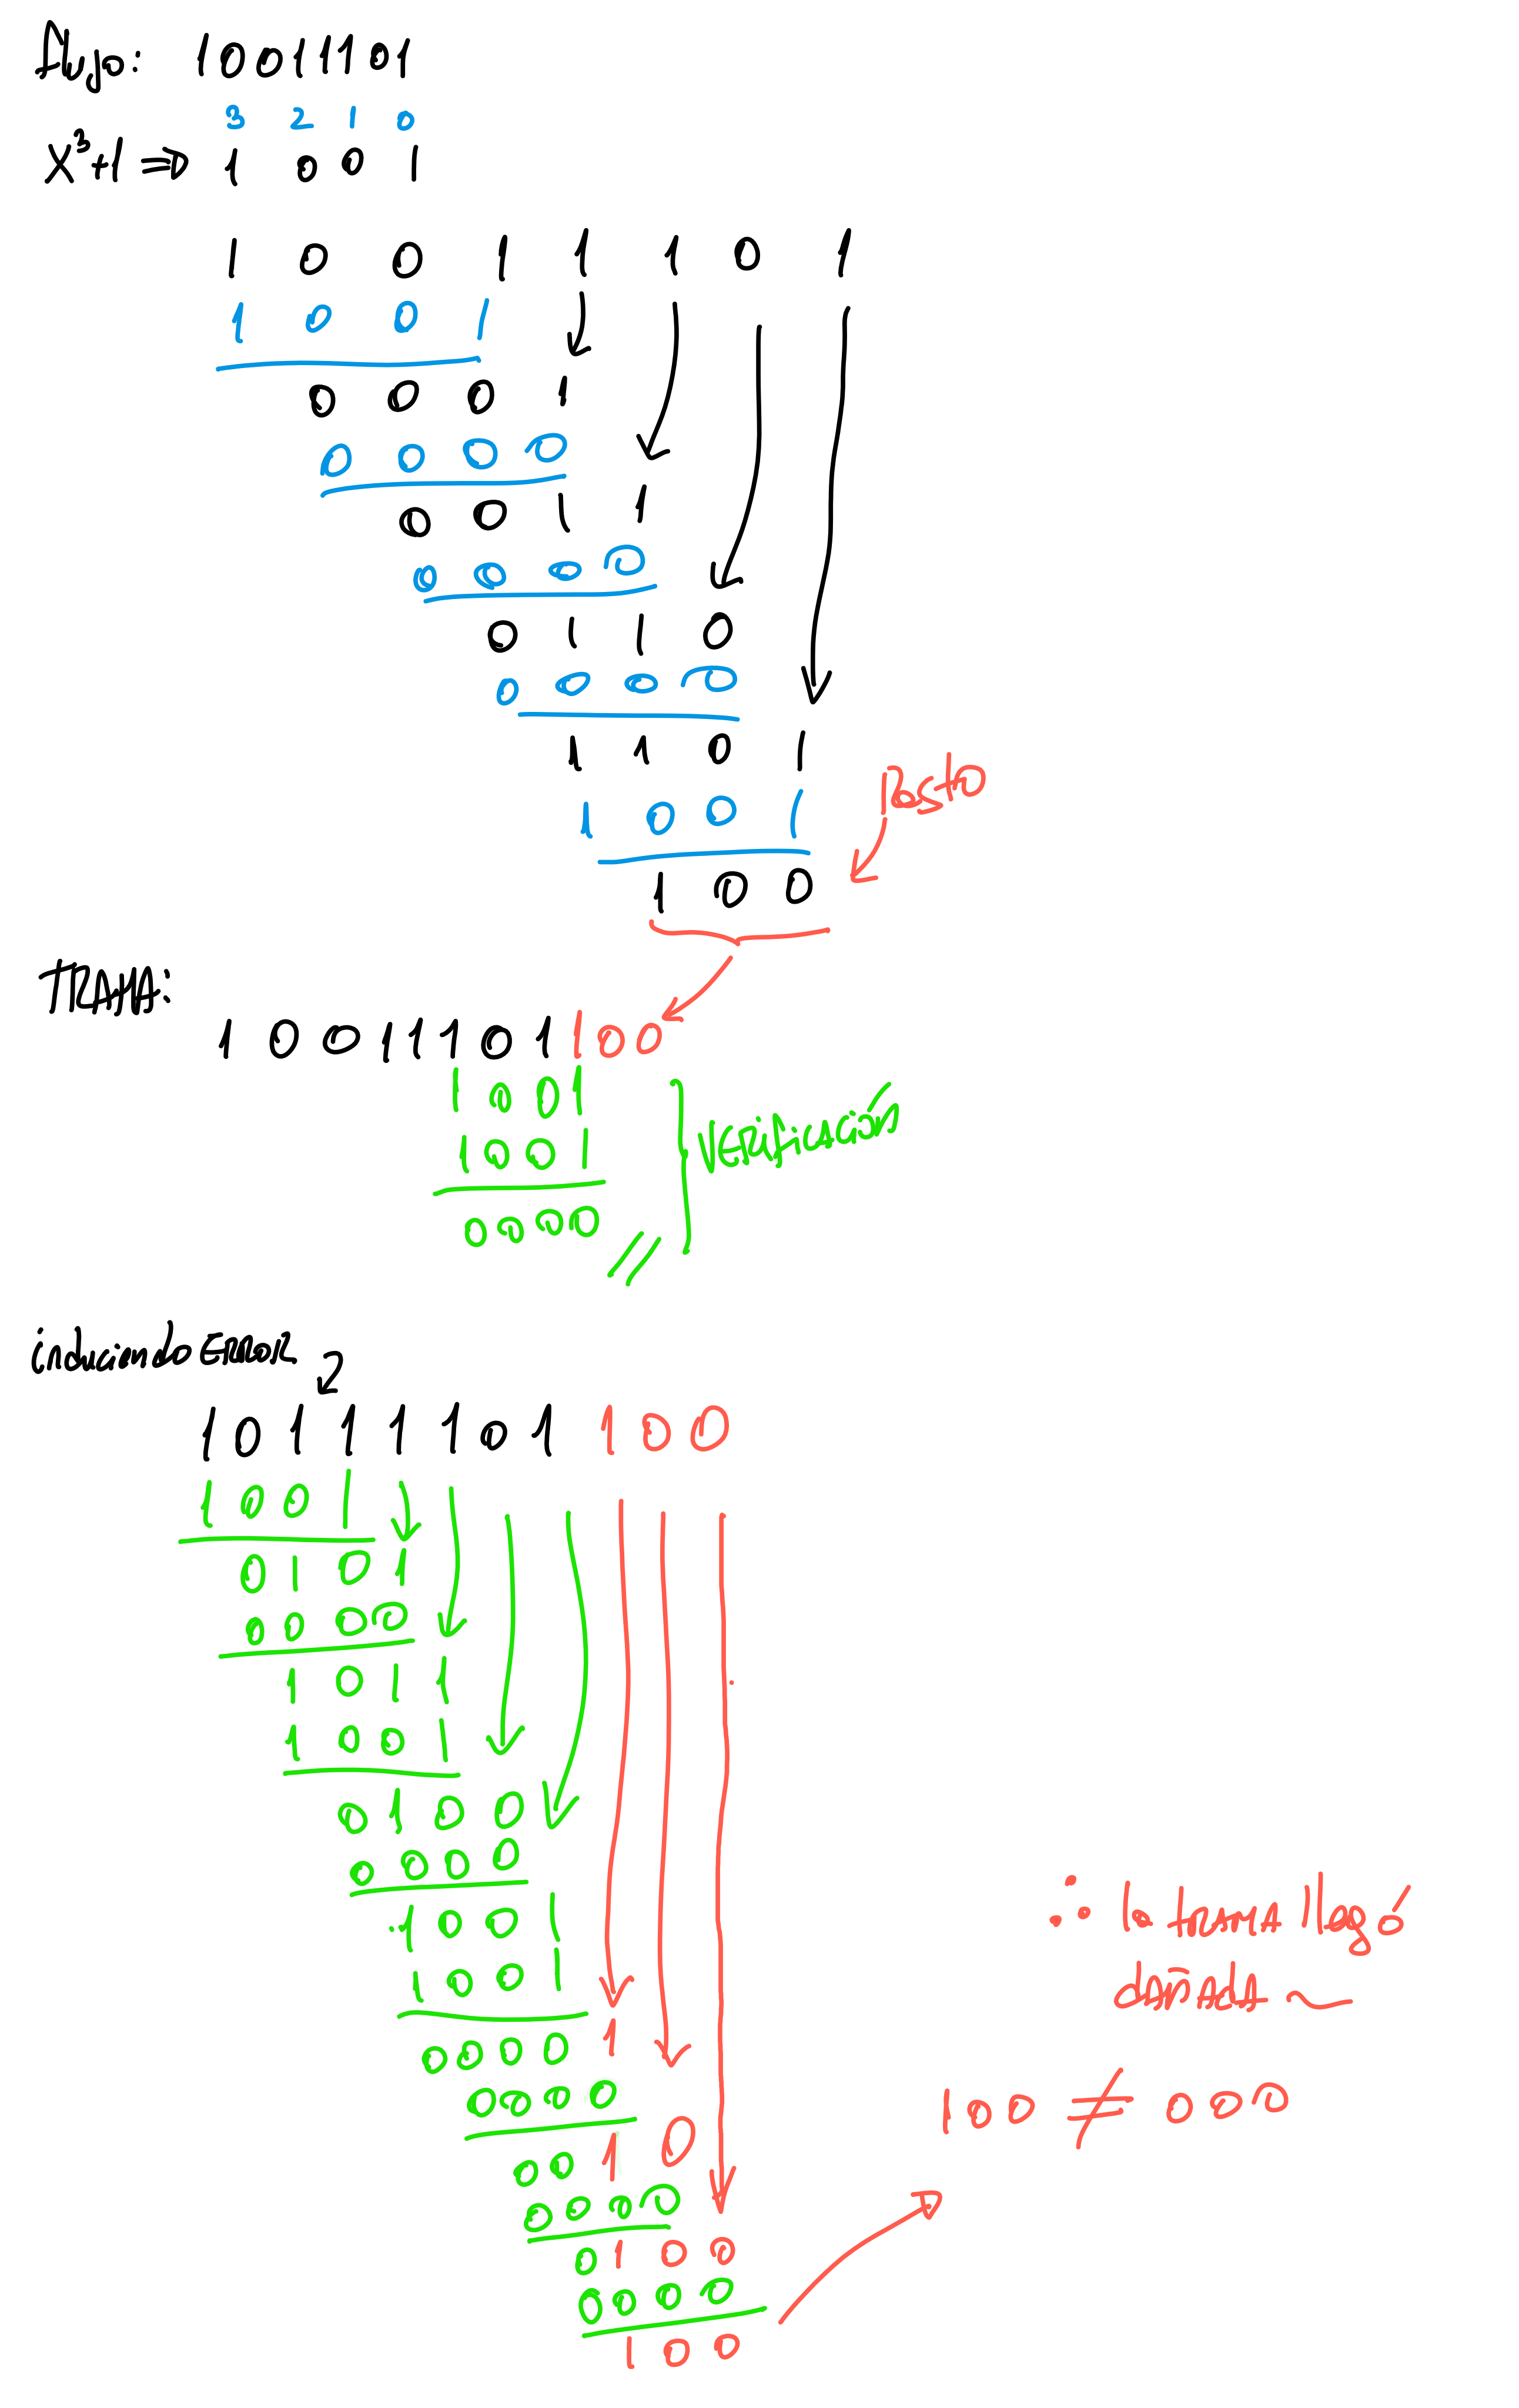
\includegraphics[height=.6\textheight]{images/2}\\
	\caption{Resolución 2}
	\label{FIG:resolucion2}
\end{figure}


\subsection{NOTA: En conjunto con el informe, deberá subir los volúmenes creados en cada actividad, por lo cual deberá considerar que el tamaño de estos sea lo menor posible. Las actividades que no cuenten con todos los archivos necesarios para su comprobación, será valoradas como actividades
	fallidas, por lo tanto, evaluadas con cero puntos.}
Están incluidas en el bundle.

\subsection{En el informe de laboratorio deberá explicar, con sus palabras, cómo funciona el sistema de cifrado que realiza Veracrypt. Además deberá investigar qué tipos de errores se pueden detectar con CRC, los polinomios generadores más comunes y en que capa del modelo OSI se aplica.}

VeraCrypt pertenece a la categoría de herramientas para el encriptado "al-vuelo" y este puede encriptar una particion completa o bien crear un archivo como volumen para ser montado como una. Puede usar una amplia variedad de algoritmos de encriptado -los cuales están listados dentro del manpage- y utiliza XTS como mecanismo. El mecanismo de cifrado funciona a grandes razgos por medio del encriptado de los datos utilizando una llave, luego esta llave se lleva a un lugar de la memoria (usualmente al comienzo) para luego ser encriptado por medio de una llave externa. De esta manera la llave que posee el usuario no tiene relación algún por tamaño de bloques con los correspondientes al contenido o bien a la llave usada para el cifrado original de estos (XTS).\cite{REF:veracrypt}

CRC puede funcionar como una herramienta para verificar la integridad de los datos o bien para permitir la recuperación de estos (si es que la firma posee ciertas características).\cite{REF:crc} En este contexto, no existe tal cosa como un polinomio generador mas comun, ya que depende directamente del contexto en el cual se usa, por ejemplo, si bien tiene sentido utilizar un CRC de 32 bits en un proceso de compresión, no tiene sentido en dispositivos embebidos debido a que estos suelen tener menor capacidad de computo (por palabra)\cite{REF:mellon}. Debido a esto mismo, de asociar directamente CRC a una capa del modelo OSI esta entraría en la capa de \text{enlace de datos}  ya que es el punto donde se ejecutan movimientos de datos y es necesario verificar la integridad de los mismos.


\subsection{Además, deberá explicar cada procedimiento utilizado durante la realización de cada una de las actividades, respondiendo las preguntas y observaciones solicitadas para cada una de ellas. También deberá indicar como piensa usted que la realización de cada actividad ayuda a asegurar la confidencialidad e integridad.}

Las respuestas están \textit{inlined} en cada sección, los comandos utilizados están presentes en la carpeta \texttt{scripts} y sus resultados en \texttt{results} del bundle entregado. Siento que cada activiad per se no asegura la confianza e integridad. Desafortunadamente el problema con todas estas herramientas es su mal uso, por tanto pueden llevar a sentir al usuario dentro de una falsa sensación de seguridad. Por ejemplo, bien se puede encriptar todo el disco y agregar un volumen oculto tal y como dice el manual, pero si el tipo no tiene idea de como resguardar la información para acceder al mismo, entonces simplemente perdió la información. Es lo mismo con los usuarios que piensan que encriptando su disco duro principal estan seguros, cuando en realidad si no desactivan el modo suspensión o hibernación nada impide que se obtena un snapshot del estado de la memoria RAM. Nuevamente, falta de seguridad.

Ahora dentro de esa falsa sensación si, se pueden incluir que satisface la confidencialidad e integridad desde el punto de vista que si esta información con un disco cifrado bajo condiciones \textit{tipicas} cae en manos desconocidas, si su portador no tiene los conocimientos necesarios del entorno y de la tecnología, entonces tiene nada en sus manos. De alguna forma te hace sentir mas seguro en el caso que trabajes con información sensible y de pronto te roban el equipo o tu disco duro.

\subsection{El informe deberá contar con portada, índice y referencias.}
Ya están incluidas.

\subsection{El contenido de dicho informe no deberá sobrepasar las 10 páginas de extensión (sin contar portada, índice y referencias).}
No las sobrepasa.

\begin{thebibliography}{9}
	\bibitem{REF:crc}
	Bill McDaniel.
	\textit{An Algorithm for Error Correcting Cyclic Redundance Checks}.
	https://www.drdobbs.com/an-algorithm-for-error-correcting-cyclic/184401662, 2002.

	\bibitem{REF:gnupg}
	Linux Man pages.
	\textit{gpg(1) - Linux man page}.
	https://linux.die.net/man/1/gpg.


	\bibitem{REF:veracrypt}
	VeraCrypt.
	\textit{Documentation}.
	https://www.veracrypt.fr/en/Documentation.html.


	\bibitem{REF:mellon}
	Koopman, Philip and Chakravarty, T.
	\textit{Cyclic redundancy code (CRC) polynomial selection for embedded networks}.
	10.1109/DSN.2004.1311885. 2004.


\end{thebibliography}

\end{document}